\section{Phased broadband spectra from single chirp excitation}
\label{sec:bbqchili}

The are numerous nuclei of considerable interest to \ac{NMR} practitioners with
very wide chemical shift ranges, including \textsuperscript{13}C,
\textsuperscript{19}F -- of particular interest in the
pharmaceutical industry -- and \textsuperscript{31}P. Attaining spectra
covering the entire
chemical shift range of such spins for use in quantitative applications is
challenging due to off-resonance effects, which severely alter the amplitudes
and phases of resonances with frequencies far from the transmitter
frequency\cite[Section 3.4.1]{Cavanagh2007}. One popular means of achieving
\emph{broadband} excitation, in which a consistent amplitude- and phase-profile
across the spectral window the achieved, is to use swept-frequency (chirp)
pulses, whose excitation frequency varies with
time\cite{Bohlen1989,Bohlen1993}.
The application of a single \ang{90} chirp pulse to achieve broadband
excitation, while simple, yields spectra with undesirable phase behaviour, on
account of resonances with different frequencies being excited at different
moments during chirp application. However, with knowledge of the form of the
chirp pulse, the expected phase of a particular resonance is determinable, and
can be corrected with appropriate post-processing.

In this section, a description of a method given the name \ac{BBQCHILI} is
presented, which provides a means of acquiring well-phased broadband spectra
from single chirp excitation. \ac{BBQCHILI} comprises two key steps: (a)
estimation of the acquired \ac{FID}'s parameters, (b) generation of a synthetic
\ac{FID}, with each contributing oscillator being back-propagated by an
appropriate amount, according to its resonance frequency. A description of the
technique is presented, followed by an illustration of its performance on
simulated and experimental datasets.

\subsection{An overview of single chirp excitation}
Here, focus is limited to chirp pulses whose frequency varies linearly with
time, which sweep from low to high frequencies. Such a pulse is defined by its
duration $\tau_{\text{p}}$ (\unit{\second}),
excitation bandwidth $\Updelta F$ (\unit{\hertz}),
and \ac{RF} amplitude $\nu_{\text{RF}}$ (\unit{\hertz}).
The frequencies that the pulse sweeps through are in the range $\left[\foffone -
\nicefrac{1}{2} \Updelta F, \foffone + \nicefrac{1}{2} \Updelta F\right]$, and
the rate at which the frequency of the chirp is increased (the sweep rate) is
given by $\nicefrac{\Updelta F}{\tau_{\text{p}}}$.
Figure \ref{fig:single-chirp} provides an illustration of a single chirp
excitation experiment. After application of the chirp pulse, there is commonly
a short \emph{pre-scan delay} $\tau_{\text{del}}$, typically on the order of
\unit{\micro\second}, prior to the start of acquisition, which is also of
relevance in order to process the \ac{FID}.

The various pulse parameters are inter-related as follows:
\begin{equation}
    \nu_{\text{RF}} = \sqrt{
        \frac{\Updelta F Q}{2 \pi \tau_{\text{p}}}
    },
\end{equation}
where $Q \in \mathbb{R}_{>0}$ is the \emph{adiabaticity factor} \note{More
detail/citation?}. For a pulse with flip angle  $\beta < \ang{180}$,  $Q$ is
related to $\beta$ via
\begin{equation}
    Q = \frac{2}{\pi} \ln \left( \frac{2}{\cos(\beta) + 1} \right),
\end{equation}
\note{ref?}
such that an appropriate pulse to achieve a flip angle of \ang{90} requires
selecting a combination of $\nu_{\text{RF}}$, $\Updelta F$, and
$\tau_{\text{p}}$ which satisfies $Q \approx 0.441$.

\begin{figure}
    \centering
    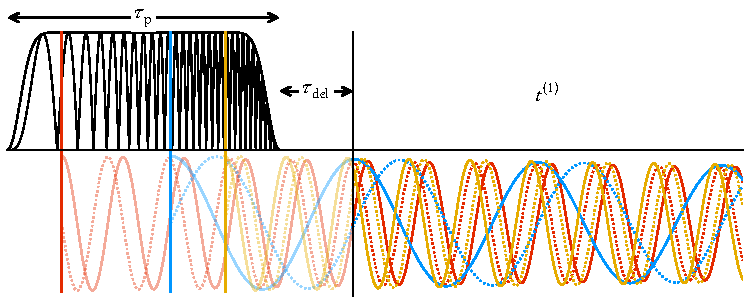
\includegraphics{single_chirp_illustration/single_chirp_illustration.pdf}
    \caption{
        An illustration of an experiment comprising a single chirp pulse sweeping
        low to high frequencies of duration $\tau_{\text{p}}$, followed by
        a pre-scan delay period or $\tau_{\text{del}}$, prior to
        acquisition. The fate of three resonances with different frequencies is
        denoted, with $\fone_{\text{red}} < \fone_{\text{blue}} <
        \fone_{\text{yellow}}$. Each resonance is excited at different points
        in time, with lower frequency resonances being excited earlier, such that
        each resonance is allowed to evolve for different amounts of time prior
        to acquisition ($t_0$).
        The resulting \ac{FID} possesses quadratic phase behaviour.
        Coloured oscillations denote the evolution of each resonance, with
        solid and dashed lines representing real and imaginary components,
        respectively. It is assumed that the \ang{90} chirp rotates each
        resonance to be initially in phase with the receiver.
    }
    \label{fig:single-chirp}
\end{figure}

For a pulse with sufficiently low $\nu_{\text{RF}}$ (which in turn requires a
sufficiently large $\tau_{\text{p}}$ for a given excitation bandwidth) it is
valid to assume that the chirp induces an instantaneous \ang{90} rotation
of a spin at the point of resonance. As such, resonances with different
frequencies evolve for different amounts of time prior to the start of
acquisition, according to
\begin{equation}
    t_0\left( \fone \right) =
        \tau_{\text{del}} + \frac{\tau_{\text{p}}}{2} -
        \frac{\left( \fone - \foffone \right) \tau_{\text{p}}}{2 \Updelta F}.
    \label{eq:t0}
\end{equation}
$\tau_{\text{del}} + \nicefrac{1}{2} \tau_{\text{p}}$ is the amount of time
between excitation and detection for an on-resonance oscillator. Resonances
with an frequency smaller than the transmitter are excited earlier and hence
have a larger $t_0$, while the converse is true for resonances with greater
frequencies. An illustration of this phenomenon is provided by Figure
\ref{fig:single-chirp}.

\subsection{Quadratic phase correction and \acs{BBQCHILI}}
Appropriate phasing of the spectrum generated via single chirp excitation can
be reduced to a trivial zero-order problem by applying phase correction
(Section \ref{subsec:nmr-analysis}), with \note{Check $2 \pi$}
\begin{equation}
    \phi \left( \fone \right) =
        \underbrace{
            2 \pi \left(\fone - \foffone\right) \left(\tau_{\text{del}}
            + \frac{\tau_{\text{p}}}{2} \right)
        }_{\phi_1} -
        \underbrace{
            2 \pi \left(\fone - \foffone\right)^2 \left(
            \frac{\tau_{\text{p}}}{2 \Updelta F} \right)
        }_{\phi_2}.
    \label{eq:quadratic-phase}
\end{equation}
While \eqref{eq:quadratic-phase} is able to correct the quadratic phase
behaviour of peaks, it is unable to address another issue with the dataset,
which is the fact that for each resonance, a number of initial points are not
present in the \ac{FID}.
For any resonance, the signal that is actually detected can be thought of as
the difference between two signals: (a) the ``complete'' signal, which starts
at the time of excitation, and (b) a ``truncated'' signal which is identical to
the complete signal before acquisition, and which comprises zeros once
acquisition has begun. The linear nature of the \ac{FT} dictates that the
resulting delayed-acquisition spectrum comprises the difference between the
\acp{FT} of the complete signal and the truncated signal.  The \ac{FT} of the
truncated \ac{FID} is well approximated as a broad sinc wiggle with its maximum
at the resonance frequency. The form of the wiggle depends on the delay between
excitation and acquisition, with resonances of lower frequencies, for which
more of the signal is missed, displaying deeper, and narrower artefacts. The
result of applying quadratic phase correction is therefore a spectrum of
well-phased peaks, but with severe baseline distortion, particularly to the
right-hand (low frequency) end. Panel b of Figure
\ref{fig:chirp-phase-vs-backprop} provides an example of this phenomenon.

Both quadratic phase and missing point-derived baseline distortions can be
resolved if an estimate of the \acp{FID} parameters is obtained. Estimation
opens up the means of constructing \iac{FID} featuring oscillators which
are back-propagated, such that they begin not at the point of acquisition, but
at the point of excitation. The appropriate start time for an oscillator with
frequency $\fone$ is therefore given by $-t_0\left( \fone \right)$, with  $t_0$
defined in \eqref{eq:t0}. The resulting corrected \ac{FID} $\by_{\text{corr}}$
is as follows:
\begin{equation}
    \begin{split}
        \by_{\text{corr}} \left[ \none \right] =
            &\sum_{m=0}^{M-1} \bdam \exp \left( \iu \bdphim \right) \times \\
            &\exp\left(-
            \left(2 \pi \iu \left(\bdfonem - \foffone \right) - \bdetaonem \right)
            t_0 \left(\bdfonem\right) \none \Dtone
            \right).
    \end{split}
\end{equation}
Estimation can be carried out using the \ac{MPM}, with the option of applying
\ac{NLP} afterwards. However, the variance of oscillator phases should not be
included in the fidelity for \ac{NLP}, since the phases in the dataset are
quadratically distributed. For the examples presented in this work, the direct
output of the \ac{MPM} was used.

\begin{figure}
    \centering
    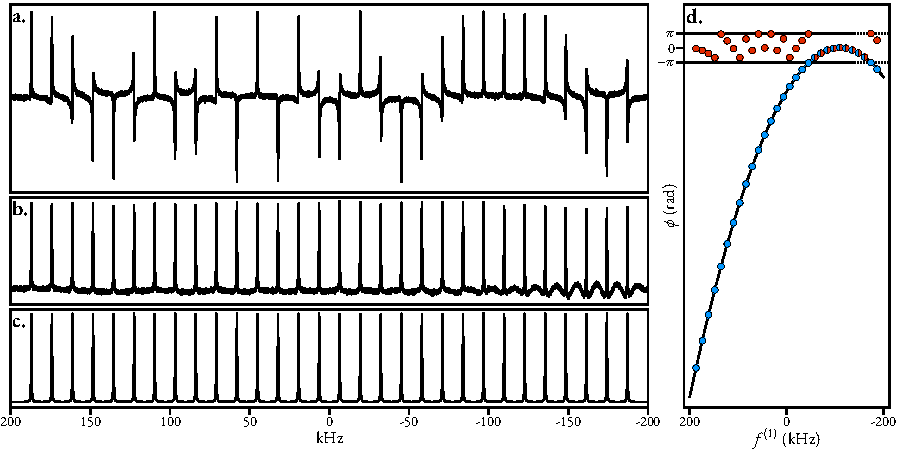
\includegraphics{chirp_phase_vs_estimation/chirp_phase_vs_estimation.pdf}
    \caption[
        Comparison of quadratic phase correction vs frequency-dependent
        back-propagation in treating data derived from a single-chirp
        excitation experiment.
    ]
    {
        Comparison of quadratic phase correction vs frequency-dependent
        back-propagation in treating data derived from a single chirp
        excitation experiment.
        \textbf{a.} Simulated spectrum for a spin system comprising 30 spins
        with uniformly-separated resonance frequencies. The data was generated
        with
        $\None=2^{15}$,
        $\fswone=\qty{500}{\kilo\hertz}$,
        $\foffone=\qty{0}{\hertz}$,
        $\tau_{\text{p}} = \qty{100}{\micro\second}$,
        $\tau_{\text{del}} = \qty{0}{\second}$,
        $\Updelta F = \qty{500}{\kilo\hertz}$.
        \textbf{b.} Spectrum generated using quadratic phase correction, with
        \eqref{eq:quadratic-phase}.
        \textbf{c.} Spectrum generated from estimation using the \ac{MPM}, and
        back-propagation.
    }
    \label{fig:chirp-phase-vs-backprop}
\end{figure}
